\Exercise Estudieu el grup de simetria d'aquest objecte (trobeu elements i operacions de simetria i construïu la taula)

\begin{center}

\includegraphics[scale=0.4]{../figures/logoMercedes.jpg}
\end{center}

\Answer Comencem per identificar les isometries, les transformacions que deixen la figura invariant. El logo té tres eixos de simetria (veure figura) i també dues rotacions ($R_0^{2\pi/3}$ i $R_0^{4\pi/3}$). Finalment hem de considerar també la transformació identitat, $Id$.

\begin{center}
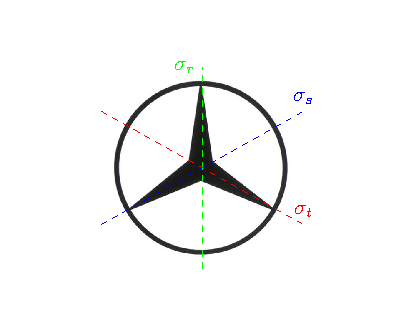
\includegraphics[width=0.8\linewidth]{../figures/simetriaMercedes.pdf}
\end{center}

a partir d'aquesta informació podem construir la taula de composició d'isometries, cosa que, entre altres, ens permet visualitzar si hem oblidat alguna altra isometria:

\begin{center}
\begin{tabular}{|>{\columncolor{gray}}c|c|c|c|c|c|c|}
  \hline
  \rowcolor{gray}
  $\circ$         & $Id$          & $\sigma_r$      & $\sigma_s$      & $\sigma_t$    & $R_0^{2\pi/3}$ & $R_0^{4\pi/3}$  \\\hline
  $Id$            & $Id$          & $\sigma_r$      & $\sigma_s$      & $\sigma_t$    & $R_0^{2\pi/3}$ & $R_0^{4\pi/3}$  \\\hline
  $\sigma_r$      & $\sigma_r$    & $Id$            & $R_0^{4\pi/3}$  & $R_0^{2\pi/3}$ & $\sigma_t$    & $\sigma_s$      \\\hline
  $\sigma_s$      & $\sigma_s$    & $R_0^{2\pi/3}$   & $Id$            & $R_0^{2\pi/3}$ & $\sigma_r$    & $\sigma_t$      \\\hline
  $\sigma_t$      & $\sigma_t$    & $R_0^{4\pi/3}$  & $R_0^{4\pi/3}$  & $Id$          & $\sigma_s$    & $\sigma_r$      \\\hline
  $R_0^{2\pi/3}$   & $R_0^{2\pi/3}$ & $\sigma_s$      & $\sigma_t$      & $\sigma_r$    & $R_0^{4\pi/3}$& $Id$            \\\hline
  $R_0^{4\pi/3}$  & $R_0^{4\pi/3}$& $\sigma_t$      & $\sigma_r$      & $\sigma_s$    & $Id$          & $R_0^{2\pi/3}$   \\\hline
\end{tabular}
\end{center}

De l'observació de la taula es pot trobar la isometria inversa de cada element del grup. De la transformació al voltant d'un eix de simetria, la inversa és ella mateixa, la qual cosa es coneix com la propietat involutiva, ja que la doble transformació duu a la identitat:
\[
\sigma_s \circ \sigma_s =Id
\]
Pel que fa als girs, l'un és l'invers de l'altre:
\begin{eqnarray*}
  (R_0^{2\pi/3})^{-1} &=& R_0^{4\pi/3}\\
  (R_0^{4\pi/3})^{-1} &=& R_0^{2\pi/3}\\
\end{eqnarray*}
També observem que el grup no és commutatiu, ja que, per exemple, $\sigma_s \circ \sigma_t \neq \sigma_t \circ \sigma_s$.
